\documentclass[../main.tex]{subfiles}

\begin{document}

\section{Discussion}

Our CRNN model underperformed, achieving 61\% test accuracy compared to the 
baseline ResNet's 79\%. This is likely due to the dataset's simplicity, which 
led the RNN layers to overfit and reduced generalization.

CRNN's strength in modeling spatial and temporal features was underutilized, as 
fixed spectrogram window sizes likely limited effective temporal capture. 
Meanwhile, the baseline ResNet, optimized for spatial features, was sufficient for 
emotion classification without relying on temporal data.

\subsection{Performance Along Other Dimensions}

Switching to a simpler CNN model improved test accuracy to 75\%. This is because 
CNNs excel at handling static image data, like spectrograms, by focusing on 
spatial patterns and structures without the complexity of temporal dependencies. Thus, 
classification performance is improved when the model focuses on the task of 
image processing.

\begin{figure}[h]
    \centering
    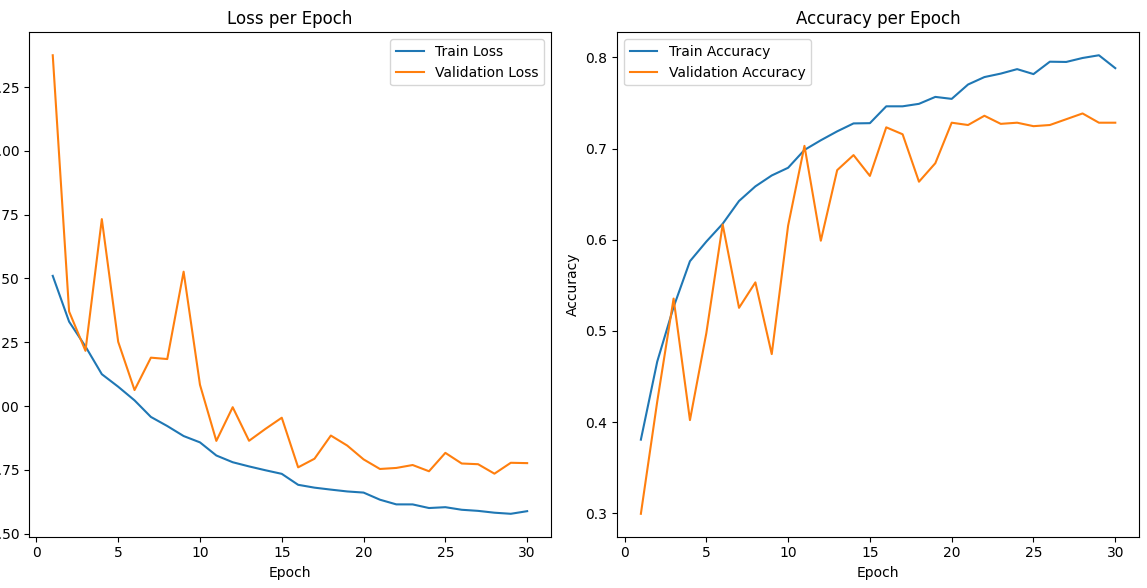
\includegraphics[width=.5\linewidth]{../resources/cnn_mixed.png}
    \caption{Loss and accuracy of traing and validation data of a CNN model.}
    \label{fig:cnn_mixed}
\end{figure}

\subsection{Training Using TESS/CREMA-D but Testing on RAVDESS}

To test real-world performance, we trained our CRNN on TESS and CREMA-D 
and tested on RAVDESS, achieving only 25\% accuracy. Most predictions were 
classified as "angry" due to differing voice patterns in RAVDESS. This 
suggests our model, with limited training data, wouldn't generalize well 
in real-world scenarios.

\begin{figure}[ht]
    \centering
    \begin{minipage}{.5\textwidth}
      \centering
      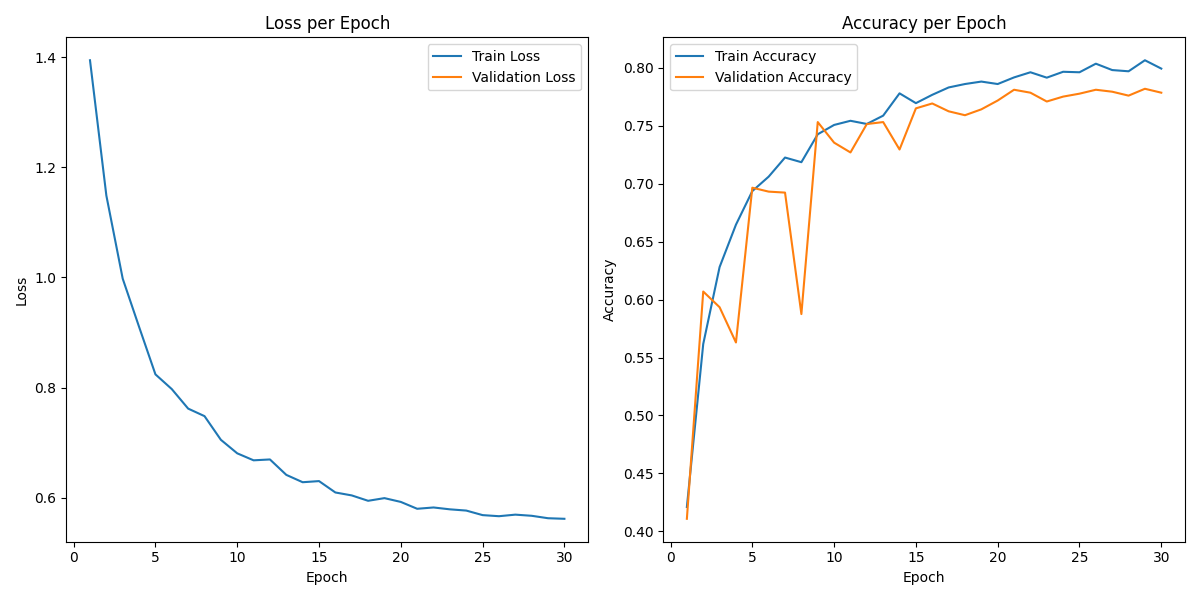
\includegraphics[width=1.0\linewidth]{../resources/cnn_unmixed.png}
      \caption{Loss and accuracy of training and validation of CNN model trained on 
      TESS and CREMA-D and tested on RAVDESS.}
      \label{fig:cnn_unmixed}
    \end{minipage}%
    \hfill
    \begin{minipage}{.4\textwidth}
      \centering
      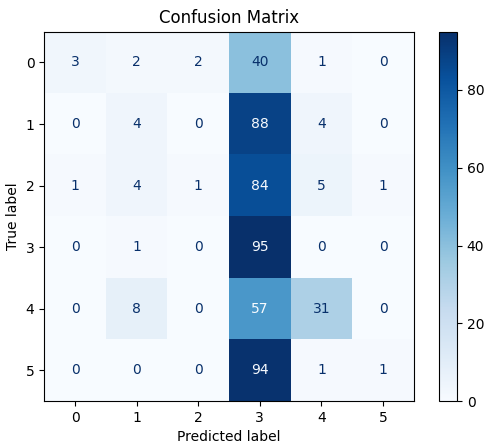
\includegraphics[width=.8\linewidth]{../resources/cnn_unmixed_confusion.png}
      \caption{Confusion matrix of CNN model trained on TESS and CREMA-D 
      and tested on RAVDESS. The categories are the same as 
      \autoref{fig:baseline_confusion}.} 
      \label{fig:cnn_unmixed_confusion}
    \end{minipage}
\end{figure}

\subsection{Overfitting With the TESS Dataset}

Training and testing our CRNN on just the TESS dataset yielded 99\% accuracy, 
thanks to its balanced yet homogeneous samples from only two speakers. However, 
when using three datasets (TESS, CREMA-D, RAVDESS), the model struggled to 
generalize across varied recording conditions, speakers, and emotions, leading 
to more average performance.


\end{document}